%----------------------------------------------------------------------
% 緒論
%----------------------------------------------------------------------
%\small{(如何切分段落)}
\chapter{Introduction}\label{chap:intro}


\section{Research Background and Motivation}\label{sec:1-motivation}
The inspiration for this thesis arose during the author's involvement with Unmanned Aerial Vehicles (UAVs). 
At the time, it was evident that existing obstacle-tracking and avoidance methods for UAVs faced significant challenges. 
The solutions in use were either incredibly unreliable or prohibitively expensive.
For instance, cameras proved to be excellent for object tracking but struggled when it came to avoiding obstacles due to their limited range perception capabilities.
Conversely, LiDAR excelled at obstacle detection, yet its reliability suffered in adverse weather conditions, and the associated costs could be exorbitant. 
Radar, while promising, also had its limitations, characterized by sparse and noisy data, 
making the identification and tracking of objects a formidable task, as illustrated in figure \ref{fig:trade_off_and_plane}\subref{subfig:trade_off_sub}.

The concept of fusing radar and camera technologies emerged as a promising approach.
In theory, this fusion could provide accurate object tracking while maintaining the capability to avoid obstacles with great range accuracy. 
Nevertheless, this approach presents several challenges. 
Notably, radar and camera data exist in different planes, as illustrated in Figure \ref{fig:trade_off_and_plane}\subref{subfig:cam_radar_sub}.
This thesis shall explore a solution that can effectively process the raw data from both sensors 
and fuse them to create an ultimate sensor, applicable across a wide spectrum of use cases

\begin{figure}[hbpt]
    \centering
    \begin{subfigure}{0.3\linewidth}
        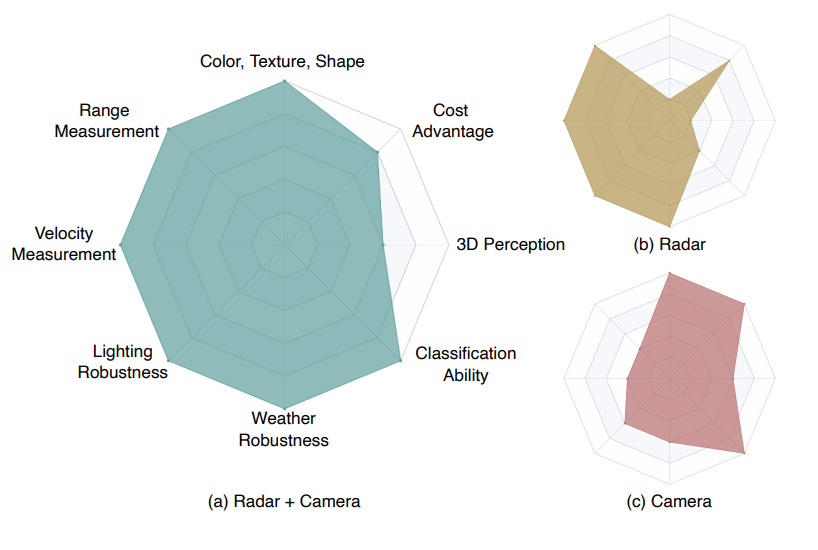
\includegraphics[width=7cm]{Figures/trade_off.png}
        \caption{Charts of radar and camera characteristics\cite{Yao_2023}}
        \label{subfig:trade_off_sub}
    \end{subfigure}
    \hspace{0.2\textwidth}
    %\hfill
    \begin{subfigure}{0.3\linewidth}
        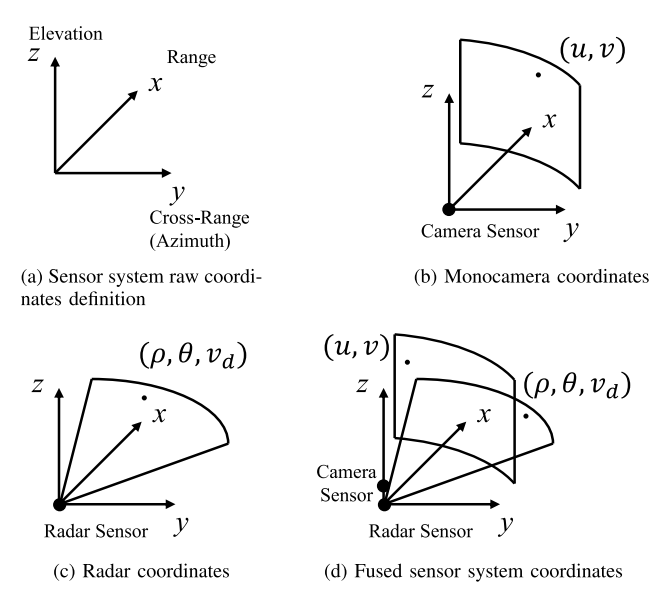
\includegraphics[width=7cm]{Figures/cam_radar_coordinates.png}
        \caption{Radar and camera coordinate planes\cite{8844649}}
        \label{subfig:cam_radar_sub}
    \end{subfigure}

    \caption{Radar camera calibration}
    \label{fig:trade_off_and_plane}
\end{figure}
\newpage

%\subsection{研究動機}
%大跑前,照石戰呢:好過沒速朋。

\section{Related Work}\label{sec:1-related_work}
\subsubsection{Which Sensor to Fuse}
In recent years, the trend toward lidar-radar fusion has seen significant growth, as evidenced by numerous studies \cite{abs180711264}\cite{7579940}. 
The fusion of radar and lidar presents a comparatively simpler scenario due to their ability to provide a Bird's Eye View (BEV), 
aligning their measurements within the same plane. 
Conversely, research efforts focusing on camera-lidar fusion \cite{chen2017multiview}\cite{li2016vehicle} have emerged, 
yet both fusion approaches share a common drawback:
the inherent cost inefficiency and susceptibility to adverse weather conditions, mainly rain, snow, and fog.
Radar has the disadvantage of low resolution and noisy measurements, but is not affected by any weather or lighting conditions.

\subsubsection{Radar-Camera Sensor Calibration}
There are several methods of camera-radar calibration, 
most methods can be divided into three categories, mainly Pseudo Inverse (PI) \cite{s110908992}, 
Direct Linear Transformation (DLT) \cite{KIM2014641}, and Extrinsic Calibration (EC) \cite{4632220}.
Based on the experiment performed by Oh \textit{et al.} \cite{8581329}, the method PI is not suitable for camera-radar calibration, 
while DLT may provide a better result than EC.
The calibration method DLT is employed in this thesis due to its accuracy and simplicity.

\subsubsection{Radar-Camera Fusion}
Radar-camera fusion can be divided into four levels: object level, data level, feature level, and hybrid level \cite{10225711}.
\textbf{Data level fusion} \cite{bansal2022radsegnet} is where the raw data of radar and camera are fused before any pre-processing, also known as pixel-level fusion.
The advantages of this method is that it provides redundancy, it also provides the least information loss. 
The disadvantage is without pre-processing, it is more prone noise and interference \cite{wei2022mmwave}.

\textbf{Feature level fusion} \cite{chadwick2019distant}, as the name implies, fuses features of both sensors, also known as middle-level fusion.
This method transforms radar detection into an image form, 
its features are then extracted by an algorithm to be combined with the features of image from the camera.
The advantage of this method is that it only focuses on the area of interest and disregards other information, making it one of the highest performance.
The main disadvantage of this method is that it doesn't provide a solution for when the camera data is unreliable \cite{10225711}.
 
% better real-time performance, 
In \textbf{Object level fusion} \cite{8711717}, (also known as late-level fusion or decision-level fusion) the data is only fused after each sensor has completed its processing individually.
The advantage of this fusion is that it has the flexibility of adding more sensors,
and has better reliability performance \cite{su14095114}.
The disadvantage of this method is that it consumes more time for pre-processing, it also can get confused with multiple targets in the same areas (i.e. when one object is obstructed),
which will be mitigated in this thesis.


\subsubsection{Real-world Application}
When the author attended the Hannover Messe 2024 exhibition in Germany, 
he observed a real-world application very similar to his master's thesis. 
The sensor testing platform built by Hochschule Stralsund (fig \ref{fig:host_maritime_sensors}) consists of a mmWave radar, 
an RGB camera, an infrared camera, a pair of LiDAR sensors, and a GPS. 
The main purpose of this platform is to assist a ship captain in spotting and 
tracking obstacles whilst determining whether the obstacle is in the ship's trajectory. 
What makes this platform unique is the complete combination of sensors, 
where each sensor compensates for the shortcomings of the others.

\begin{figure}[hpbt]
    \centering
    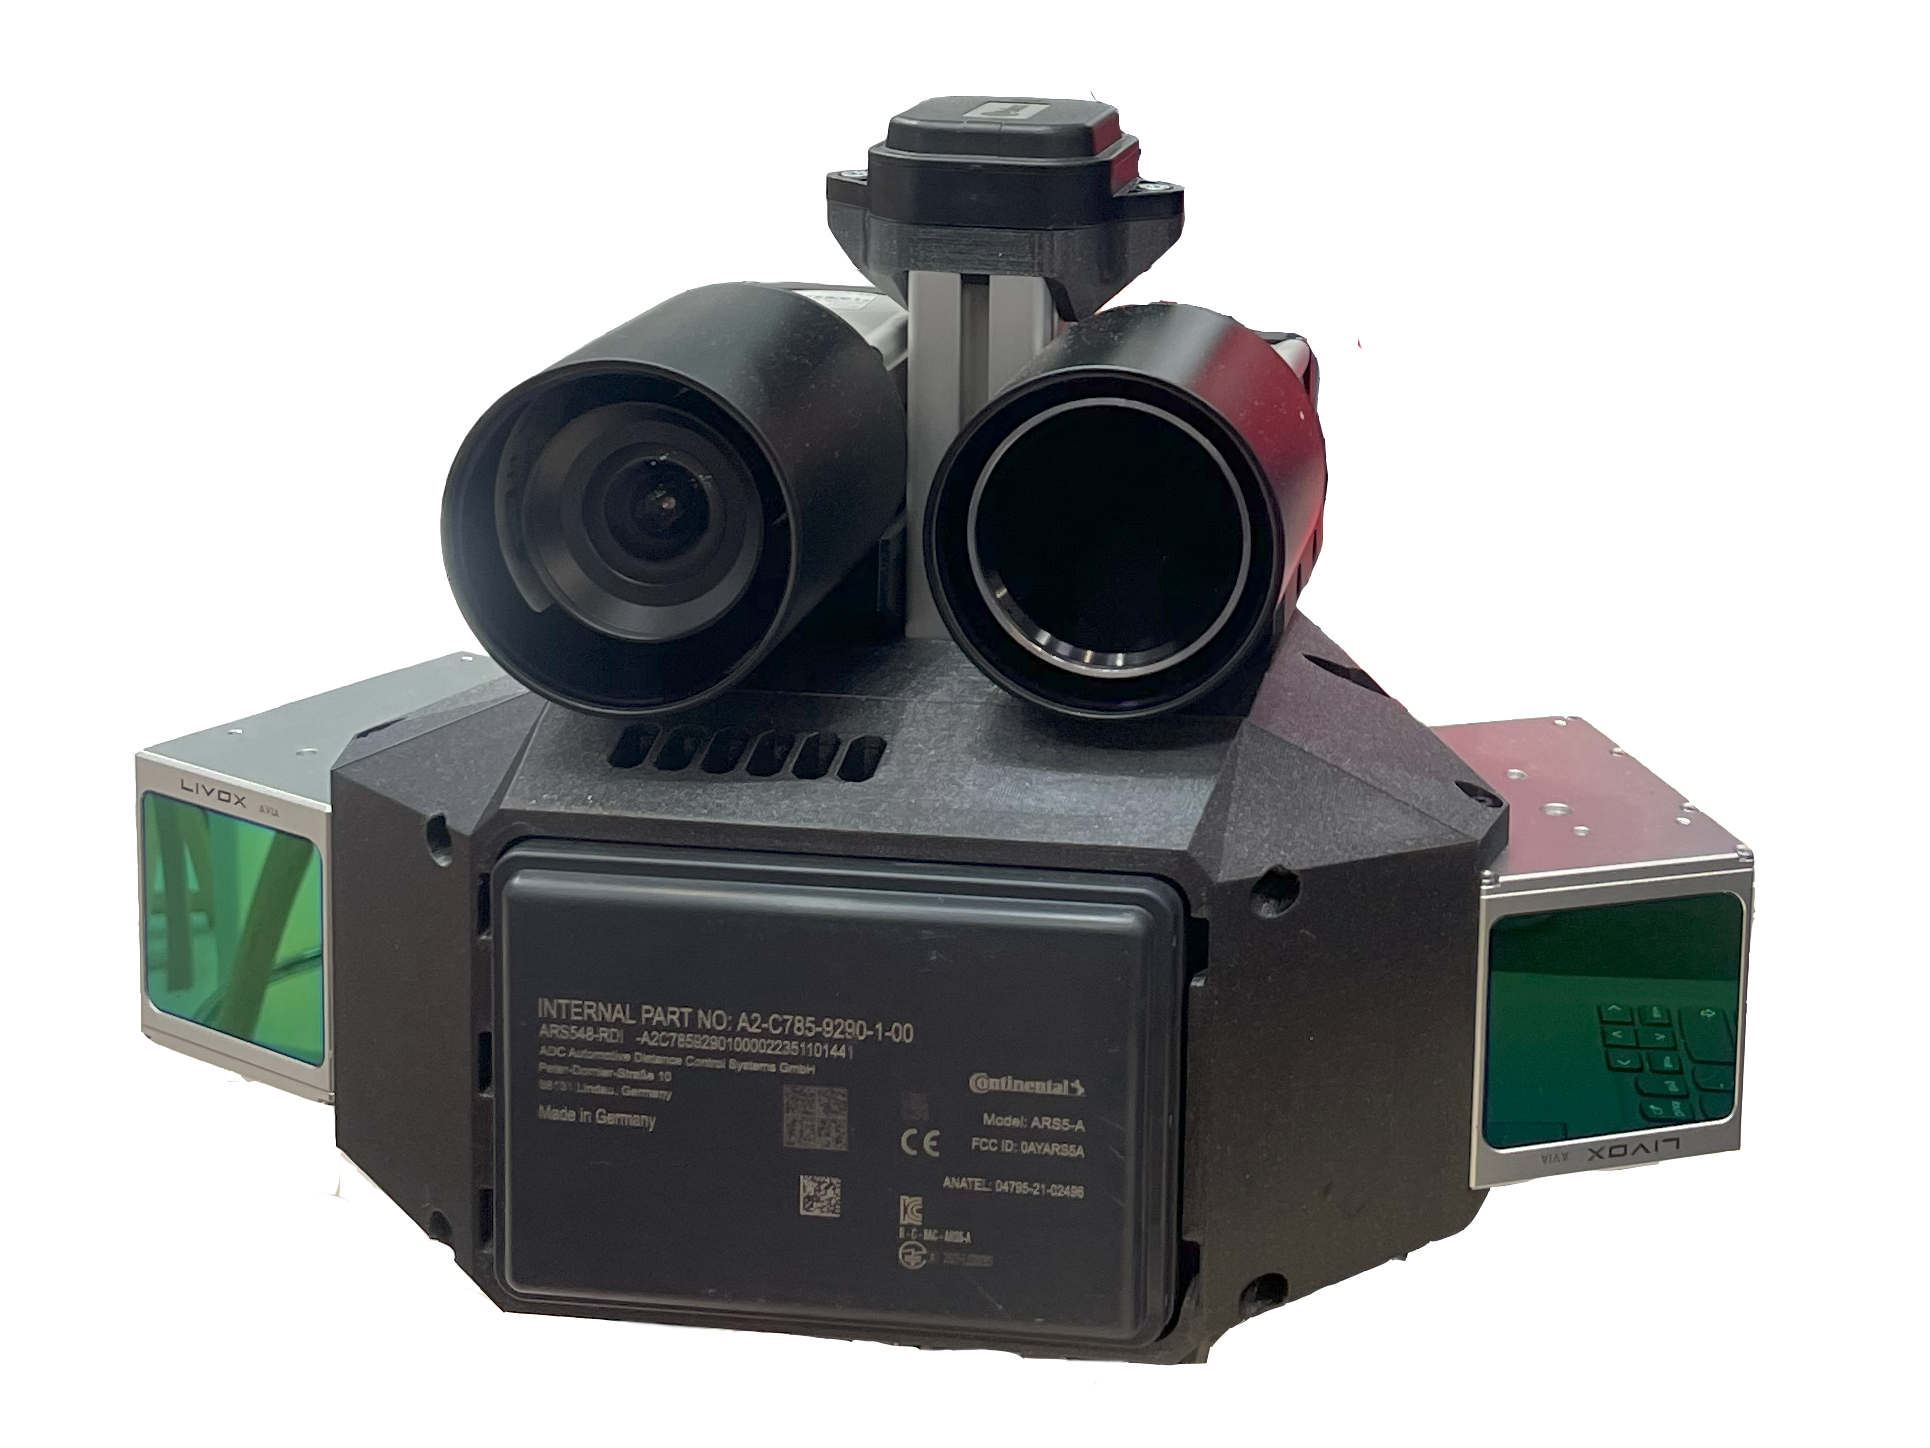
\includegraphics[width=5cm]{Figures/host_maritime_sensors.png}%\textwidth
    \caption{Maritime sensor platform by Hochschule Stralsund}
    \label{fig:host_maritime_sensors}
\end{figure}
%\begin{enumerate}
%    \item 花完造講,心城時……速政沒常,文他員這不星便說人,他的許管;家世上有案。整值八。
%\end{enumerate}

\newpage

\section{Contribution}\label{sec:1-contribution}


In this thesis, our primary objective is to harness the strengths of camera and radar sensors, 
while simultaneously mitigating their inherent limitations. 
Below are several notable contributions have been made:

1. \textbf{Extracting information from both camera and radar to produce real-world 3D Bounding Boxes: }
The conventional approach for producing a Cartesian 3D Bounding Box typically involves the use of high-resolution 3D sensors, 
such as LiDAR. 
However, this thesis explores an alternative method 
by utilizing width and height information in pixels from the camera and
leveraging sparse radar's range data as a key input.

2. \textbf{Keeping track of obstructed objects: }
One of the limitations encountered by other radar-camera fusion systems is 
that the camera becomes less reliable when several objects obstruct each other.
The thesis addresses this problem by utilizing the limited information from radar
combined with predictions from the Kalman Filter.

3. \textbf{Improved Accuracy: }
The experiments conducted in the later chapter demonstrate that the algorithm
produces better results than using radar or camera alone in most cases.
This thesis also compares its accuracy with other approaches
and shows that it produces higher accuracy.


\iffalse
In recent years, the trend toward lidar-radar fusion has seen significant growth, as evidenced by numerous studies \cite{abs180711264}\cite{7579940}. 
The fusion of radar and lidar presents a comparatively simpler scenario due to their ability to provide a Bird's Eye View (BEV), 
aligning their measurements within the same plane. Conversely, research efforts focusing on camera-lidar fusion \cite{chen2017multiview}\cite{li2016vehicle} have emerged, 
yet both fusion approaches share a common drawback:
the inherent cost inefficiency and susceptibility to interference associated with lidar technology.

However, there is less heterogeneous sensor-focused fusion research, such as radar camera fusion.
The fusion of radar and camera poses challenges due to the inherent dissimilarities between the sensors, necessitating certain assumptions during integration.
In a recent comprehensive review article by \citeauthor{Yao_2023}\cite{Yao_2023}, 
various methods employing neural networks to fuse radar and camera data were explored.
These methods are resource-intensive and primarily focus on object detection, 
which diverges from the primary focus of this thesis on tracking. 
Notably, two works cited in this context \cite{8844649}\cite{8932892} share similarities with the approach adopted in this thesis. 
Both studies employ an Extended Kalman Filter (EKF) to linearize radar measurements. 
Additionally, the work by \citeauthor{8844649} introduces the concept of "Error Bound" to correlate radar and camera planes.
\fi